\documentclass[a4paper,11pt]{report}
\usepackage[T1]{fontenc}
\usepackage[utf8]{inputenc}
\usepackage{graphicx}
\usepackage{underscore}
\usepackage[italian]{babel}

\newcommand{\HRule}{\rule{\linewidth}{0.5mm}}


\begin{document}
\thispagestyle{empty}
\pagestyle{empty}

\begin{center}
\textsc{Universitità di Cagliari}\\[0.4cm]
\textsc{Facoltà di Scienze MM.FF.NN.}\\[5.5cm]

\textbf{{\large Tesina Corso SO1 - Parte 2, Threads}}\\[0.6cm]
Davide Gessa (45712)\\[0.4cm]
\textit{A.A. 2011 - 2012\\[0.4cm]}

\vfill
\textit{28 Dicembre 2011\\[1.5cm]}


\end{center}

\newpage
\tableofcontents


\chapter{Struttura del programma}

\section{Suddivisione files}
Il codice del programma è stato ripartito in vari file cercando di dividere le varie 
funzionalità dei diversi "oggetti della scena":

\begin{itemize}
  \item alien.c alien.h - navicella aliena
  \item bomb.c bomb.h - bomba aliena
  \item control.c control.h - controllo delle iterazioni tra i vari oggetti e rendering della scena
  \item main.c - starter dell'applicazione
  \item missile.c missile.h - missile lanciato dall'astronave
  \item scores.c scores.h - gestione dei punteggi
  \item space_ship.c space_ship.h - navicella giocatore
  \item utility.c utility.h - funzioni varie utili per il funzionamento del programma
  \item space_invaders.c space_invaders.h - definizioni globali e funzioni comuni
\end{itemize}

\section{Elenco funzioni}
\begin{itemize}
  \item alien_task() : gestione navicella aliena
  \item bomb_task() : gestione bomba aliena
  \item clear_quad() : cancella un area quadrata dello schermo
  \item control_check_collision() : controlla se c'è una collisione tra due oggetti
  \item control_task() : gestione della scena
  \item missile_task() : gestione di un missile
  \item render_string_array() : renderizza uno sprite nello schermo
  \item scores_add() : aggiungi un punteggio alla lista punteggi
  \item scores_load() : carica i punteggi da un file
  \item scores_save() : salva i punteggi in un file
  \item space_ship_task() : gestione navicella giocatore
  \item timevaldiff() : calcola la differenza tra due strutture timeval
  \item queue_add() : aggiunge un elemento alla coda di update
  \item queue_get_first() : restituisce il primo elemento della coda di update
  \item queue_init() : inizializza la coda di update
  \item queue_exit() : deinizializza la coda di update
  \item get_free_object_index() : restituisce la prima posizione libera nel buffer condiviso degli oggetti
  \item control_set_collision() : imposta ad un oggetto lo stato delle collisioni
  \item get_collision_state() : restituisce ed azzera lo stato delle collisioni di un oggetto
\end{itemize}


\section{Il main}
La funzione main si preoccupa di inizializzare l'applicazione (coda di update, dimensione schermo), creare i thread per gli oggetti iniziali con
le relative funzioni di gestione.

\begin{enumerate}
  \item Creazione thread navicella
  \item Creazione dei threads degli alieni
  \item Avvio della funzione di controllo
\end{enumerate}




\chapter{Architettura del programma}

Ogni oggetto segue un funzionamento simile agli altri oggetti, e viene creato nel medesimo modo; ogni oggetto ha
una funzione di gestione così strutturata:
\begin{enumerate}
  \item Inizializza i dati iniziali e li inserisce in una struttura di tipo object_data_t
  \item Esegue un loop (dal quale esce al verificarsi di alcune condizioni) che ad ogni iterazione 
    produce le nuove informazioni dell'oggetto (ad esempio, tramite la tastiera nel caso
    della navicella del giocatore), le inserisce nella sua struttura e le invia
    al controllo tramite una coda di update. Inoltre, il controllo può utilizzare il buffer condiviso
    per segnalare ad un determinato oggetto che è avvenuta una collisione (vedi sezione \ref{sec:comun}).
\end{enumerate}

Le informazioni di un oggetto sono memorizzate nella seguente struttura: 

\begin{verbatim}
///> Struttura contenente le informazioni relative all'oggetto
typedef struct
{
	int 			x;			///< Posizione x dell'oggetto
	int				y;			///< Posizione y dell'oggetto
	int 			size;		///< Dimensione dell'oggetto (sia x che y)
	
	object_type_t	type;		///< Tipo di oggetto
	int				life;		///< Vita rimanente all'oggetto
	
	pthread_t		thread;		///< Thread assocciato all'oggetto
	int				id;			///< Posizione nell'array degli oggetti
	
	direction_t		dir;		///< Direzione oggetto (usata per i marzianetti)
	
	
	pthread_mutex_t coll_mutex;	///< Mutex per aggiornare le collisioni
	object_type_t	coll;		///< Stato delle collisioni dell'oggetto
} object_data_t;
\end{verbatim}

Strutturare in questo modo il software, mi ha consentito di convertire la versione che utilizzava i processi/pipe, nella versione
corrente che utilizza i threads in meno di un ora; mi è bastato aggiungere delle funzioni thread-safe per la gestione della comunicazione,
e sostituirle alle vecchie chiamate per la scrittura/lettura delle pipe.

\section{Comunicazione dei Task} \label{sec:comun}
Per quanto riguarda la comunicazione tra il task di controllo e gli oggetti, ho strutturato il software 
in modo da diminuire il numero di accessi in memoria ed i tempi di attesa ai semafori; 
tutti gli oggetti della scena condividono:

\begin{itemize}
  \item objects[OBJECTS_MAX] : Un buffer contenente tutti gli oggetti della scena con le relative informazioni, nel quale ci scrive 
        il thread di controllo per segnalare agli oggetti eventuali collisioni. 
        Il controllo utilizza la funzione control_set_collision(object_data_t *obj, object_type_t t) 
        per segnalare ad un oggetto 'obj' che è avvenuta una collisione con un oggetto di tipi 't'; l'informazione verra inserita nell'apposito
        slot dell'array 'objects'.
        Il thread dell'oggetto, potrà verificare se sono avvenute collisioni con la funzione object_type_t get_collision_state(int id).
  \item queue[QUEUE_SIZE] : Una coda di update nella quale gli oggetti inseriscono la loro struttura object_data_t per essere renderizzata 
        dal controllo. E' possibile accedere alla coda 'queue' tramite delle apposite funzioni che permettono di sincronizzare gli accessi:
          queue_add(object_data_t ob) : aggiunge un oggetto alla coda (usata dai thread degli oggetti)
          queue_get_first(object_data_t *ob) : preleva un oggetto dalla coda (usata dal controllo per ottenere il prossimo oggetto da renderizzare)
\end{itemize}


Una schematizzazione della comunicazione tra i task dell'applicazione è visibile in figura 2.1.

\begin{center}
\begin{figure}
\begin{center}
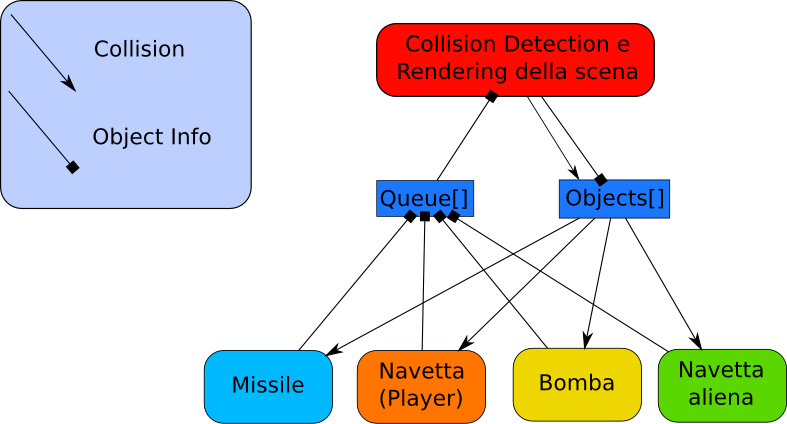
\includegraphics[scale=0.70]{comunication.png}
\end{center}
\caption{Schema di comunicazione fra i tasks}
\end{figure}
\end{center}

\section{Tasks}
Come stabilito nelle specifiche, alieni, controllo, bombe, navicella e missili utilizzano
un thread separato ciascuno.

\subsection{Controllo}
Il thread di controllo esegue un loop, ed ad ogni iterazione si occupa di:
\begin{enumerate}
  \item Ricevere dalla coda 'queue' le informazioni relative ad un oggetto
  \item Salvare nell'array 'objects' le informazioni ricevute
  \item Controllare se l'oggetto è in collisione con un altro oggetto, ed in tal caso, eseguire una control_set_collision per informare l'oggetto
  \item Cancellare l'area di schermo occupata dall'oggetto nell'iterazione precedente
  \item Ridisegnare l'oggetto nella nuova posizione
\end{enumerate}
Il ciclo viene interrotto quando si verifica una condizione di gameover, o quando il giocatore vince.
Quando il gioco finisce, il controllo invia a tutti i threads ancora in vita (missili, bombe, alieni, navicella) 
un informazione (tramite buffer condiviso) per avvisare che il programma deve chiudersi e che i threads devono terminare.

Finito il gioco, viene aggiunto il punteggio nella lista punteggi salvata in un file, e viene visualizzata
la classifica.

\subsection{Alieno}
Si muove seguendo un percorso destra->giu->sinistra->giu come nel gioco originale;
ad ogni iterazione invia al controllo la nuova posizione tramite la coda, e legge dal buffer condiviso 
degli oggetti le informazioni relative alle collisioni:
se collide con un altro alieno, cambia direzione, altrimenti decrementa
la vita, e nel caso abbia finito le vite disponibili, si distrugge e si ricrea di livello superiore.

Ad intervalli regolari l'alieno sgancia una bomba, generando un nuovo thread.

\subsection{Bomba}
Il thread bomba ad ogni iterazione, scende di una posizione, invia al controllo la nuova posizione tramite la coda, e legge dal buffer condiviso 
degli oggetti le informazioni relative alle collisioni.

\subsection{Navicella}
Ad ogni iterazione, il thread della navicella attende un input da tastiera per comandare il movimento
o sparare dei missili; il movimento può essere solo orizzontale. 
Il lancio dei missili è limitato da un timer, che permette un certo numero di spari ogni secondo.
Premuto il tasto di sparo, la navicella crea due nuovi threads (missile destro e missile sinistro)
che avviano la funzione di gestione del missile.

\subsubsection{Missile}
Il thread missile ad ogni iterazione, sale di una posizione in verticale, si sposta di un'unità in
orizzontale (a seconda che sia un missile destro od un missile sinistro), invia le info al controllo tramite la coda, e attende
un tempo predefinito; come per la bomba, il loop termina quando il processo di controllo segnala un avvenuta collisione
con un altro oggetto.


\section{Sincronizzazione}
Avendo due buffer condivisi da tutti i threads, ho dovuto sincronizzare gli accessi per non generare inconsistenze nei dati.

\subsection{Buffer 'objects'}
E' possibile accendervi per modificare lo stato delle collisioni; ogni elemento del buffer contiene un mutex 'coll_mutex' ed una variabile
intera 'coll'; per modificare la variabile intera 'coll' è necesssario fare un lock del mutex.
Ho realizzato due funzioni threadsafe per modificare e leggere il contenuto della variabile coll, control_set_collision() per impostare una 
collisione ad un oggetto e get_collision_state() per verificare lo stato delle collisioni di un oggetto e azzerarne il valore.

\subsection{Coda 'queue'}
E' possibile accedervi per inserire un oggetto in coda o per prelevare il primo inserito tramite le due funzioni queue_add() e queue_get_first();
ho utilizzato l'algoritmo per il buffer condiviso, con n produttori ed un consumatore; le due funzioni sopra citate utilizzano tre semafori per regolare l'accesso al buffer.


\end{document}
